\chapter{最適輸送問題の予備知識} \label{ch:optimal-transport}

本研究内で偏微分方程式の解法に用いるthe back-and-forth methodについて説明する。

\section{最適輸送}
\label{sect:最適輸送}
\subsection{Mongeの最適輸送問題}
\label{sect:Mongeの最適輸送問題}
back-and-forth methodは本来最適輸送問題を求めるアルゴリズムである。
まず、最適輸送問題について説明する。
1781年、G.Mongeによって最適輸送問題が提唱された。

\begin{monge}
    ある砂山から砂山(測度$\mu$)と同じ体積の穴(測度$\nu$)に砂を運ぶ(写像$T$)。
    輸送にかかるコストは重さと移動距離に依存する時,コストを最小にする方法を求めよ。
\end{monge}

最適輸送問題を数学的に解釈するため、押し出し測度(pushforward measure)を定義する。
\begin{dfn}
    $\mu$ から $\nu$ へ輸送する写像を$T$とするとき$(T_\#\mu = \nu)$,
    押し出し測度は
    \begin{equation*}
        \nu (A) =  T_\#\mu (A) := \mu (T^{-1} (A)) \qquad A \subset \Omega
    \end{equation*}
    で定義される(\ref{fig:pushforward measure})。
    また、押し出し測度をテスト関数$f: \Omega \to \mathbb{R}$に対する押し出し測度eの積分として定義すると以下のようになる:
    \begin{equation}
        \label{def:pushforward_int}
        \int_{\Omega} f(y)d\, T_\# \mu (y) = \int_\Omega f(T(x)) d \mu(x).
      \end{equation}
\end{dfn}

\begin{figure}[htbp]
    \label{fig:pushforward measure}
    \begin{center}
        \includegraphics[width=0.8\textwidth]{images/transport_map2.JPG}
        \caption{輸送写像}
    \end{center}
\end{figure}

上記の押し出し測度を用いて最適輸送問題の定式化を行う。

\begin{monge}
    $\Omega \subset \mathbb{R}^d$を凸集合とし、
    $c : \Omega \times \Omega \to \mathbb{R}$を$x$から$y$への輸送コストを表すコスト関数、
    $\mu, \nu : \Omega \to \mathbb{R}$を$\Omega$上の確率測度、
    $T : \Omega \to \Omega$を写像とする。
    ここで$T_\#\mu = \nu$は、測度$\mu$を$\nu$に変換することを意味する。

    $\mu$から$\nu$への輸送の最小コストは、$C(\mu, \nu)$で表され、次のように計算される:

    \[
    C(\mu, \nu) = \int_{\Omega} c(x, T(x)) \,dx
    \]
\end{monge}

\subsection{Kantorovich双対問題}
\label{sect:Kantorovich双対問題}
最適コスト$C$は、輸送の位置を固定するのではなく、輸送される砂の体積を最大化する問題として考えることができる。
この考えはKantorovichによって導入された。\cite{MR0096552}
これをKantorovich双対問題という。


\begin{Kantorovich}
$\mu$と$\nu$が確率測度であり、$c(x, y)$が$x$から$y$への輸送コストを表す場合、コスト$C$は以下のように、砂を輸送する体積を最大化する問題として表現できる:
\[
    C(\mu, \nu) = \sup_{\varphi, \psi} \left( \int \varphi \,d\nu + \int \psi \,d\mu \right)
\]
ここで、$\varphi(x)$および$\psi(y)$はKantorovich ポテンシャルであり、以下の不等式を満たす:
\[
    \varphi(x) + \psi(y) \leq c(x, y)
\]
\end{Kantorovich}
{\color{red}
ここで、多孔質媒体方程式は固定された$m > 1$に対して、エネルギー関数$U(\rho) = \frac{1}{m - 1} \int \rho^m \, dx$に基づくWasserstein 勾配流として表現できる。
ただし、2-Wasserstein距離のKantorovichの双対公式は次のように表される:

\begin{equation}
    \label{eq:wasserstein dual}
    \frac{1}{2\tau} W_2^2(\rho, \mu) = \sup_{(\varphi, \psi) \in \mathcal{C}} \left( \int \varphi d\rho + \int \psi d\mu \right),
\end{equation}

ここで、$\mathcal{C}$は制約
\[
    \mathcal{C}  := \{(\varphi, \psi) \in C(\Omega) \times C(\Omega) : \varphi(x) + \psi(y) \leq \frac{1}{2 \tau} |x - y|^2 \}. 
\]
を満たす関数$(\varphi, \psi)$の集合、$\tau$はスキーム内の時間ステップを表す。
}


Mongeの最適輸送問題を直接解く代わりにKantorovich双対問題を解くことで、最適写像を求めることができる。
双対問題を解く利点として以下3点があげられる。
\begin{itemize}
    \item 圧力変数$\varphi$は密度変数$\rho$よりも正則性が高いため、離散的な近似スキームに適している。
    \item 双対汎関数の微分を計算するための明示的な式があるため、勾配上昇法で解くことができる。
    \item 双対問題は制約のない形で表現されるため、厳しい制約を持つ問題にも適用できる。    
\end{itemize}

back-and-forth methodはこの2-Wasserstein距離におけるKantorovich双対問題を解くことで最適写像を求める。

\section{c-変換(c-transform)}
\label{sect:c-変換(c-transform)}
ここではc-変換に必要な数学の知識を踏まえ、c-変換を導入する。
\subsection{凸包(convex hull)}
\label{sect:凸包(convex hull)}
\begin{dfn}[凸集合]
    $\mathbb{R}^n$の部分集合 $X$ が\textit{凸集合}であるとは、すべての $x, y \in C$ および $\forall \theta \in [0, 1]$ に対して次が成り立つときである:
    \[
        \theta x + (1 - \theta )y \in X
    \]
\end{dfn}

\begin{dfn}
    集合 $X \subset \mathbb{R}^n$ の凸包(convex hull)とは、$X$ を含む(唯一で)最小の凸集合を指し、$conv X$と表す。

\end{dfn}

\begin{dfn}
    関数 $f$ が \textit{proper} であるとは、少なくとも一つの $x \in $ に対して $f(x) < +\infty$ であり、
    すべての $x \in $ に対して $f(x) > - \infty$ であるときをいう。
\end{dfn}

\begin{dfn}(下半連続)
    関数 $f: \mathbb{R}^n \to \mathbb{R} \cup \{+ \infty\}$ とし、$x^{\prime}$ を $f$ の収束点とする。
    このとき、$f$ が $x^{\prime}$ で下半連続であるとは、次が成り立つことである:
    \[
        \liminf_{x \to x^{\prime}} {f(x)} \ge f(x^{\prime}) \quad \text{または} \quad \liminf_{x \to x^{\prime}} {f(x)} = f(x^{\prime}) 
    \]
\end{dfn}

\begin{dfn}
    $\mathcal{C}$が凸集合であるとき、関数 $f \in \mathcal{C}$ が$C$上で\textit{凸関数}であるとは、次が成り立つ場合に限る:
    \[
        f((1 - \lambda)x + \lambda y) \le (1 - \lambda) f(x) + \lambda f(y), \quad \forall x, y \in \mathcal{C}, \quad \lambda \in [0, 1].
    \] 
\end{dfn}

任意の関数$f$を凸関数とし、$f \in \mathcal{C} \ne \emptyset$とする。
$f$を$\mathcal{C} \subset \mathbb{R}^n$に含まれない点では$f(x) = +\infty$として$\mathbb{R}^n$に拡張する。
このとき、上記の定義は次の定義と等しい。

\begin{dfn}
関数$f: \mathbb{R}^n \to \mathbb{R} \cup \{+ \infty\}$が、常に$+ \infty$でない場合、および任意の$\bm{x}, \bm{y} \in \mathbb{R}^n$、$\lambda \in [0, 1]$ に対して次が成り立つとき、$f$は凸関数である。
\[
f((1 - \lambda)\bm{x} + \lambda \bm{y}) \le (1 - \lambda) f(\bm{x}) + \lambda f(\bm{y})
\]
さらに、$f: \mathbb{R}^n \to \mathbb{R}$に対して、$f$が凹関数ならば$-f$は凸関数である。
\end{dfn}

\begin{dfn}
    $f: \mathbb{R}^n \to \mathbb{R} \cup \{ +\infty\},  C \subset \mathbb{R}^n$ とする。
    この時$f$のepigraphを次のように定義する:
    \[
    \text{epi} f := \{(\bm{x},  y) \, | \, \bm{x} \in C,  y \in \mathbb{R},  y \ge f(\bm{x}) \}.
    \]
    ここで注意として、$f(x) = +\infty$は$x \notin C$のときである。
\end{dfn}


関数 \( f : \mathbb{R}^n \to \mathbb{R} \) に対して、凸包の概念も同様に存在する。
$conv f$は$f$よりも大きくない最大の凸関数である。
ここで、関数 $f: \mathbb{R}^n \to \mathbb{R}$ が関数 $g: \mathbb{R}^n \to \mathbb{R}$ によってmajorizeされるとは、
すべての $x$ に対して $f(x) \leq g(x)$ であることを指す。
また、$conv f$はすべての凸関数 $g \leq f$ の点ごとの上限(pointwise supremum)であり、点ごとの上限は凸関数である。
すなわち、
\[
    conv f = \sup_g \{ g \le f | g \text{ is convex function}\}
\]
と表すことができる。

上記を踏まえ、凸包のアルゴリズムAlgorithm\ref{al:convex hull algorithm}に示す。



\begin{algorithm}[tb]
    \caption{convex hull algorithm}
    \label{al:convex hull algorithm}
    \begin{algorithmic}[1]
        \State \textbf{Input:} array $x, y$ (coordinates of function $f$)
        \State $l = \{(0, -\infty)\}$ 
        \For {i, (nx, ny) in enumerate(zip(x(1:),y(1:)))}
            \While{True}
                \State $pi, pv \gets l(-1)$
                \State $v = \frac{ny - y(pi)} {nx - x(pi)} $
                \If{$v \le pv$}
                    \State $l \gets l(:-1)$
                \Else
                    \State $l \gets l \, \cup \, (i+1, v)$
                    \State \textbf{break}
                \EndIf
            \EndWhile
        \EndFor
        \State \textbf{return} $l$
    \end{algorithmic}
\end{algorithm}

凸包のアルゴリズムは以下のアイデアに基づいている:
\begin{enumerate}
    \item $l = \{(0, - \infty)\}$($x$座標の添字番号と2点によって作られる直線傾きを保存する) 
    \item 傾き更新(繰り返し)
    \begin{enumerate}
        \item 「一つ前の傾き$(pv)$」$ < $「現在の傾き$(v)$」$\Rightarrow$ $l$に$x$座標の添字番号$(i)$と傾き$(v)$を追加
        \item 「一つ前の傾き$(pv)$」$ > $「現在の傾き$(v)$」$\Rightarrow$ $l$から一つ前(配列$l$の最後の要素)の$x$座標の添字番号$(pi)$と傾き$(pv)$を消去
    \end{enumerate}
\end{enumerate}

例として、$x \in [1,5]$の関数$f$の凸包を考える。
\begin{equation*}
    f(x)=
    \begin{cases}
        x - 1 & \text{if $1 \le x \le 2$,} \\
        -3x + 7 & \text{if $2 \le x \le 3$,} \\
        3x - 11 & \text{if $3 \le x \le 4$,} \\
        -x + 5 & \text{if $4 \le x \le 5$.}
    \end{cases}
\end{equation*}
この時、凸包のアルゴリズムの流れは以下のようになる。
\begin{enumerate}
    \item 初期条件$l = [(0, -\infty)]$ (図\ref{convex_hull0})。
    \item $pv(=- \infty) < v(=1)$より、$l = [(0, -\infty), (1,1)]$ (図\ref{convex_hull1})。
    \item $pv(= 1) \ge v(=-3)$より、$l$から$(1, 1)$を消去。$l = [(0, -\infty)]$ (図\ref{convex_hull2}, \ref{convex_hull3})。
    \item $pv(=- \infty) < v(=-1)$より、$l = [(0, -\infty), (2,-1)]$ (図\ref{convex_hull4})。
    \item $pv(=- 1) < v(=3)$より、$l = [(0, -\infty), (2,-1), (3,3)]$ (図\ref{convex_hull5})。
    \item $pv(= 3) \ge v(=-1)$より、$l$から$(3, 3)$を消去。$l = [(0, -\infty), (2,-1)]$ (図\ref{convex_hull6}, \ref{convex_hull7})。
    \item $pv(=- 1) < v(=1)$より、$l = [(0, -\infty), (2,-1), (4,1)]$ (図\ref{convex_hull8})。
\end{enumerate}

\begin{figure}[htbp]
    \begin{tabular}{ccc}
      \begin{minipage}[t]{0.3\hsize}
        \centering
        \includegraphics[keepaspectratio, scale=0.3]{images/convex/convex_hull_0.png}
        \subcaption{初期状態}
        \label{convex_hull0}
      \end{minipage} &
      \begin{minipage}[t]{0.3\hsize}
        \centering
        \includegraphics[keepaspectratio, scale=0.3]{images/convex/convex_hull_1.png}
        \subcaption{$pv(=- \infty) < v(=1)$}
        \label{convex_hull1}
      \end{minipage} &
      \begin{minipage}[t]{0.3\hsize}
        \centering
        \includegraphics[keepaspectratio, scale=0.3]{images/convex/convex_hull_2.png}
        \subcaption{$pv(= 1) \ge v(=-3)$}
        \label{convex_hull2}
      \end{minipage} \\
   
      \begin{minipage}[t]{0.3\hsize}
        \centering
        \includegraphics[keepaspectratio, scale=0.3]{images/convex/convex_hull_0.png}
        \subcaption{$l$から$(1, 1)$を消去}
        \label{convex_hull3}
      \end{minipage} &
      \begin{minipage}[t]{0.3\hsize}
        \centering
        \includegraphics[keepaspectratio, scale=0.3]{images/convex/convex_hull_3.png}
        \subcaption{$pv(=- \infty) < v(=-1)$}
        \label{convex_hull4}
      \end{minipage} &
      \begin{minipage}[t]{0.3\hsize}
        \centering
        \includegraphics[keepaspectratio, scale=0.3]{images/convex/convex_hull_4.png}
        \subcaption{$pv(= -1) < v(=3)$}
        \label{convex_hull5}
      \end{minipage} \\  \begin{minipage}[t]{0.3\hsize}
        \centering
        \includegraphics[keepaspectratio, scale=0.3]{images/convex/convex_hull_5.png}
        \subcaption{$pv(= 3) \ge v(=-1)$}
        \label{convex_hull6}
      \end{minipage} &
      \begin{minipage}[t]{0.3\hsize}
        \centering
        \includegraphics[keepaspectratio, scale=0.3]{images/convex/convex_hull_3.png}
        \subcaption{$l$から$(3, 3)$を消去}
        \label{convex_hull7}
      \end{minipage} &
      \begin{minipage}[t]{0.3\hsize}
        \centering
        \includegraphics[keepaspectratio, scale=0.3]{images/convex/convex_hull_7.png}
        \subcaption{$pv(= -1) < v(=1)$}
        \label{convex_hull8}
      \end{minipage} 
    \end{tabular}
     \caption{凸包アルゴリズムの挙動(例)}
  \end{figure}


%Legendre-Fenchel transform %%%%%%%%%%%%%%%%%%%%%%%%%%%%%%%%%%%%%%%%%%%%%%%%%%%%%%%%%%%%%%%%%%%%%%%%%%%%%%%%%%%

\subsection{Legendre-Fenchel変換(Legendre-Fenchel transform)}
\label{sect:Legendre-Fenchel変換(Legendre-Fenchel transform)}
\begin{dfn}
    関数$f \in \mathcal{C}$を凸で微分可能な関数とするとき、$f$のLegendre-Fenchel transformは以下のように定義される。
    \begin{equation}
        f^*(p) := sup_x\{p \cdot x - f(x) \} 
    \end{equation}
    また、
    \begin{equation}
        (f^*)^*(x) = f^{**} (x) := sup_p\{p \cdot x - f^*(p) \}
    \end{equation}
    も同様に定義される。
\end{dfn}
ここで、
\[
    f^{**} = \text{cl(conv} f)  
\]
であることから、常に$f^{**} \le f$がわかる(証明については\cite[Thm. 11.1(p474)]{MR1491362}を参照)。

Legendre-Fenchel transformとは、凸関数のある点$(x(chi[i]), y(chi[i]))$における接線の傾き(微分)$p[j]$を求めるものである。
例として、$f(x) = \alpha |x|^2$とする。
このとき、
\begin{align*}
f^*(x) &= \displaystyle \sup_{p\in \Omega}{[x \cdot p - f(p)]} \quad (g(p) = x \cdot p - f(p))\\
           &=\displaystyle \sup_{p\in \Omega}{[x \cdot p - \alpha |p|^2]}\\
           &= \displaystyle \sup_{p\in \Omega}{[- \alpha(p^2 - \frac{1}{\alpha}xp)]}\\
           &= \displaystyle \sup_{p\in \Omega}{[- \alpha(p - \frac{1}{2 \alpha}x)^2 +  \frac{1}{4 \alpha}x^2]}\\
           &=  \frac{1}{4 \alpha}|x|^2 + \sup_{p\in \Omega}{[- \alpha(p - \frac{1}{2 \alpha}x)^2]}\\
           &= \frac{1}{4 \alpha}|x|^2 \qquad (\because  \text{$p = \frac{1}{2 \alpha}x$のとき,$g(p)$はsup.  $\Rightarrow f^*$は $p = \frac{1}{2 \alpha}x$のとき成立})\\
           &= \frac{1}{4 \alpha^2}f(x)\\
\end{align*}
よって、$\alpha = \frac{1}{2}$のとき、$f^*(x) = f(x)。$
また、$g(p)$が最大になるのは$p = \frac{1}{2 \alpha}x$のときである
$(g( \frac{1}{2 \alpha}x) = x \cdot \frac{1}{2 \alpha}x - \alpha  \frac{1}{4 \alpha^2}x^2 =  \frac{x^2}{4 \alpha} = f^*(x))$。
さらに、
$g(p) = x \cdot p - f(p)= x \cdot p - \alpha |p|^2$
であることから、
$g'(p) = 0 \Leftrightarrow x - 2 \alpha p = 0 \Leftrightarrow x - f'(p) = 0 \, (\because f'(x) = 2 \alpha x) \Leftrightarrow f'(p) = x$ 。

よって一般に、 $f(x) = \alpha |x| ^2$のとき、$f^*(p)$となる$x$は $f'(p) = x$より、ある点$p$での$f$の微分になり、 
かつ$x = f'(p) = 2\alpha p$ 。

つまり「$f^*(p)= sup_x\{p \cdot x - f(x) \} $の$x$を求めること」は 「$f'(p)$を求めること」に等しい。
よって Legendre-Fenchel transformとは,凸関数のある点$(x(chi[i]), y(chi[i])$における接線の傾き(微分)$p[j]$を求めるものである。


ここで$\alpha = \frac{1}{2}$のとき、 $f^*(x) = f(x) かつf'(p) = x = 2\alpha p = p$。

従って「$v[i]: (x(chi[i+1]), y(chi[i+1]))$と$(x(chi[i]), y(chi[i]))$を結んだ線分の傾き」$=$ 「$(x(chi[i]), y(chi[i]))$での接線の傾き(微分)」になる。
つまり、$\alpha = \frac{1}{2}$のとき、 $p$は$x$座標の分割であるので、十分小さい分割を取れば、 $p[j] = v[i]$となる$p$が必ず存在する.

特に凸関数ならば、$f^*(x)$は減少しない関数なので、$v[i]$も減少しない。
よって、$v[i] < p[j] \leq v[i+1]$となるものを見つけることができる。この時、

\begin{center}
    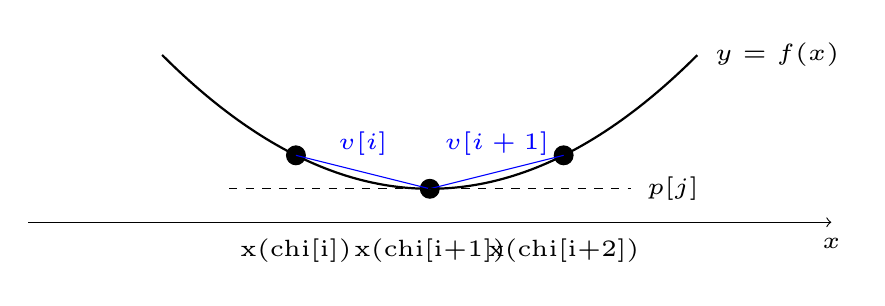
\begin{tikzpicture}[scale=1.7, transform shape]
        \label{gra:legendre}
        % グラフの描画
        \draw[->] (-3,0) -- (3,0) node[below, font=\tiny] {$x$};
        
        % 関数の描画
        \draw[black, thick, domain=-2:2, samples=100] plot (\x, {0.25*\x*\x + 0.25}) node[right, font=\tiny] {$y = f(x)$};
        
        % 点の描画
        \foreach \x/\y/\label in {-1/0.5/x(chi[i]), 0/0.25/x(chi[i+1]), 1/0.5/x(chi[i+2])}
            \filldraw (\x,\y) circle (2pt) node[below, font=\tiny] at (\x,0) {\label};
        
        % 直線の描画
        \draw[blue] (-1,0.5) -- (0,0.25) node[midway, above, font=\tiny] {$v[i]$};
        \draw[blue] (0,0.25) -- (1,0.5) node[midway, above, font=\tiny] {$v[i+1]$};
        
        % x=0での接線
        \draw[black, dashed] (-1.5,0.25) -- (1.5,0.25) node[right, sloped, font=\tiny] {$p[j]$};
        
    \end{tikzpicture}
    \captionof{figure}{Legendre Fenchel-1}
\end{center}


上記を踏まえ、Legendre-Fenchel変換のアルゴリズムAlgorithm\ref{al:legendre}に示す。

\begin{algorithm}[tb]
    \caption{Legendre-Fenchel Transform}
    \label{al:legendre}
    \begin{algorithmic}[1]
        \State \textbf{Input:} array $x, y = f(x)$ (coordinates of function $f$), $p$
        \State $chi, v \gets$ convex hull$(x, y) $
        \State $t \gets \{\}$
        \State iopt $\gets \{0,0, \dots, 0\} \quad \text{(ipot is same shape of array } x$) 
        \State $i \gets 0$
        \For {$j$, $p$ in enumerate($p$)}
            \While{$p > v(i)$}
                \State $i \gets i + 1$
            \EndWhile
            \State iopt($j$) = chi($i$)
            \State $t \gets t \cup x(\text{chi}($i$)) * p - y(\text{chi}($i$))$
        \EndFor
        \State \textbf{return} $t$, iopt
    \end{algorithmic}
\end{algorithm}

Legendre-Fenchel変換のアルゴリズムは以下のアイデアに基づいている:
\begin{enumerate}
    \item 関数$f \in \mathcal{C}$の凸包conv $f$を求める。(convex hull algorithm)
    \item 繰り返し
    \begin{enumerate}
        \item $(x(chi[i+1]), y(chi[i+1]))$と$(x(chi[i]), y(chi[i]))$を結んだ線分の傾き$v[i] \le p[j]$となる座標の添字番号$chi[i]$を見つける。
        \item $(x(chi[i]), y(chi[i]))$におけるLegendre-Fenchel変換を計算し、配列$t$に保存
    \end{enumerate}
\end{enumerate}

\subsection{$c$-変換($c$-transform)}
\label{sect:c-変換(c-transform)}
\begin{dfn}
    $\varphi$, $\psi$が$\Omega$上の連続関数の空間$\mathcal{C}(\Omega)$内の関数のとき、それぞれの$c$-変換は以下のように定義される。
    \begin{equation}
        \label{dfn:backward-c-transform}
        \psi^c(x) := \inf_{y \in \Omega} \left( \frac{1}{2\tau}|x-y|^2 - \psi(y)\right) = \frac{1}{\tau}\inf_{y \in \Omega} \left( \frac{1}{2}|x-y|^2 - \tau\psi(y)\right)
    \end{equation}
    \begin{equation}
        \label{dfn:forward-c-transform}
        \varphi^c(y) := \inf_{x \in \Omega} \left( \frac{1}{2\tau}|x-y|^2 - \varphi(x)\right) = \frac{1}{\tau}\inf_{x \in \Omega} \left( \frac{1}{2}|x-y|^2 - \tau\varphi(x)\right)
    \end{equation}
    また、 $\phi$ が $c$-凹関数とは、 $\varphi = \psi^c$ となる$\psi \in C(\Omega)$ が存在することをいう。
    さらに関数の組 $(\varphi, \psi) \in \mathcal{C}$が $c$-共役であるとは, $\varphi = \psi^c$ かつ $\psi = \varphi^c$のときをいう。
\end{dfn}


\begin{lem}
    \label{lem:c-transform}
    \hyperlink{proof:lem:c-transform}{(Proof)}
    $\varphi, \psi \in C(\Omega)$のとき、
    $\forall x \in \Omega \text{に対し,}\phi^{cc} \ge \varphi$
    が成り立つ。また、$\phi^{cc} = \varphi$の必要十分条件は$\varphi$が$c$-concaveの時である。
    ただし、$\varphi^{ccc} = \varphi^c$は常に成立する.[JL](Lemma 1(i))
\end{lem}

(proof)

$\varphi^c(p) = \frac{1}{\tau}\inf_x\left\{\frac{|x-p|^2}{2} - \tau\varphi(x)\right\}$について考える。
このときc変換は以下のようになる。
\begin{align*}
    \varphi^c(p) &= \frac{1}{\tau} \inf_x\left\{\frac{|x-p|^2}{2} - \tau \varphi(x)\right\}\\
              &= \frac{1}{\tau}  \left(\frac{|p|^2}{2} + \inf_x\left[- \left\{x \cdot p - \frac{|x|^2}{2} + \tau\varphi(x) \right\}\right]\right)\\
              &= \frac{1}{\tau}  \left(\frac{|p|^2}{2} - \sup_x\left[x \cdot p - \left\{\frac{|x|^2}{2} - \tau\varphi(x)\right\}\right]\right)\\
              &= \frac{1}{\tau}  \left(\frac{|p|^2}{2} - \sup_x\left\{x \cdot p - \psi(x)\right\} \qquad (\because \psi(x) = \frac{|x|^2}{2} - \tau\varphi(x))\right)\\
              &= \frac{1}{\tau}  \left(\frac{|p|^2}{2} - \psi^*(p)\right)\\
    \\
    \varphi^{cc}(q) 
              &= \frac{1}{\tau} \inf_p\left\{\frac{|p-q|^2}{2} - \tau \varphi^c(p)\right\}\\
              &= \frac{1}{\tau}\left(\frac{|q|^2}{2} + \inf_p\left[- \left\{p \cdot q - \frac{|p|^2}{2} + \tau\varphi^c(p) \right\}\right]\right)\\
              &= \frac{1}{\tau}\left(\frac{|q|^2}{2} - \sup_p\left[p \cdot q - \left\{\frac{|p|^2}{2} - \tau\varphi^c(p)\right\}\right]\right)\\
              &= \frac{1}{\tau}\left(\frac{|q|^2}{2} - \sup_p\left[p \cdot q - \left\{\frac{|p|^2}{2} - \left(\frac{|p|^2}{2} - \psi^*(p)\right)\right\}\right]\right)\\
              &= \frac{1}{\tau}\left(\frac{|q|^2}{2} - \sup_p\left[p \cdot q - \psi^*(p)\right]\right) \\
              &= \frac{1}{\tau}\left(\frac{|q|^2}{2} - \varphi^{**}(q)\right)
\end{align*}

上記を踏まえ、$c$-変換のアルゴリズムをAlgorithm\ref{al:c-transform}に示す。
アルゴリズムでは、$c$-変換を$\inf_x\left\{\frac{|x-p|^2}{2} - \varphi(x)\right\}$としている。
そのため、アルゴリズム中の$\varphi(x)$を$\tau\varphi(x)$、returnされた値$\frac{1}{2} p^2 - t$を$\frac{1}{\tau}\left(\frac{1}{2} p^2 - t\right)$とすることによって、実際の$c$-変換の値を計算している。

\begin{algorithm}[tb]
    \caption{c-transform}
    \label{al:c-transform}
    \begin{algorithmic}[1]
        \State \textbf{Input:} array $x,y = \varphi(x)$ (coordinates of function $f$), $p(=x)$
        \State $\psi(x) \gets \frac{1}{2} x^2 - \varphi(x)$
        \State $t$, index $\gets$ legendre-fenchel transform$(x, \psi, p)$
        \State \textbf{return} $\frac{1}{2} p^2 - t, $ index
    \end{algorithmic}
\end{algorithm}

